%Original version in April 2002 by Antje Endemann
%
%Adapted for usage in Student Conference course by jubo (050118).
%Optimized for usage with pdflatex. For usage with plain latex,
%figures must be in Postscript (.ps or .eps files) and additional
%packages must be imported.
%Last updated 100105 by jubo
%
%This template works for outline and annotated bibliography
%(deliverable 2) without any changes.
%For usage with full and final papers (deliverables 3 and 4a/b)
%you must make several changes. All necessary changes are
%described in three specific commented sections preceded by
%`%%%%% BEGIN OF ADJUSTMENTS SECTION %%%%%'.
%The changes are in order of appearance:
%   - adjust the `\documentclass' command
%   - uncomment the abstract section
%   - adjust the `\bibliographystyle' command

%%%%% BEGIN OF 1st ADJUSTMENTS SECTION %%%%%
% You must use only one of the following `\documentclass' commands
% For the outline and annotated bibliography (deliverable 2)
% you must use the following command:
%
\documentclass[runningheads,a4paper,oribibl]{llncs}
%
%For the full and final paper (deliverables 3 and 4a/b)
% you must use the command below (and put the one above in comments).
% In other words, the 'oribib' option must be used for Deliverable 2
% but not for 3 and 4a/b.
% 
%
%\documentclass[runningheads,a4paper]{llncs}
%
%%%%% END OF 1st ADJUSTMENTS SECTION %%%%%

\usepackage[T1]{fontenc}  %% needed for special characters (umlaut)
\usepackage[latin1]{inputenc}
\usepackage[swedish]{babel}
\usepackage{graphicx}     %% for graphical things such as including pictures
\usepackage{url}          %% for proper formatting of URLs

\begin{document}

\pagestyle{headings}

\mainmatter

\title{Projekt: Ultimata strategin i Paradise Hotel-finalen}

% The abbreviated title will be shown in the headers of even pages.
% You should use the full title unless it is too long.
\titlerunning{Strategi i Paradise Hotel-finalen}

\author{Johan Holmgren, Martin L�rka, Emil Edsk�r och Peter Bjuhr}

\institute{
    Department of Computing Science \\
    Ume� University, Sweden \\
    \email{id10jhn@cs.umu.se \\ id10mla@cs.umu.se \\ id10eer@cs.umu.se \\ id10pbl@cs.umu.se}
}

\maketitle

\begin{abstract}
	Here goes the actual text of your abstract. 
	������
\end{abstract}

\newpage

\section{Inledning}
Ett välkänt tv-program i Sverige, kallat “Paradise Hotel”, utser sin vinnare genom ett psykologiskt spel som spelas mellan två finaldeltagare som tilldelas varsin boll. Spelet består utav totalt 10 tidssteg, där spelarna kan välja att släppa eller att behålla bollen vid varje tidssteg. Varje tidssteg representeras av en prissumma, som ökar linjärt vid varje steg. Om båda deltagarna behåller bollen genom alla tidssteg delar de jämnt på det sista tidsstegets prissumma. Om en spelare väljer att släppa bollen på ett visst tidssteg erhåller denne hela prissumman för aktuellt tidssteg, medans motståndaren går lottlös. Med andra ord kan en spelare vinna hälften av pengarna genom att släppa bollen efter halva tiden eller genom att hålla i bollen spelet ut, men samtidigt riskera att bli blåst.

Detta projekt avser att undersöka en iterativ variant av detta spel, där spelarna möter varandra många gånger och där prissumman ersätts utav poäng. Detta är intressant eftersom de spelare som väljer att vara godtrogna vid varje spel, är de spelare som troligtvis vinner minst antal gånger samtidigt som de kammar hem fler poäng per vinst. De spelare som släpper bollen vid första tidssteget vid varje spel kommer att vinna varje gång, men antalet poäng kommer att vara mindre. Målet är att hitta den strategi som presterar bäst över tid. 15 stycken strategier (spelare) har implementerats och tävlat mot varandra. Rapporten beskriver resultatet av följande frågor:

\begin{itemize}
\item \nohyphens{Vilken strategi ger maximal utdelning om spelet körs x antal omgångar?}\\*
	\emph{Hypotes: Strategin “Tit-for-tat”, som släpper bollen ett tidssteg tidigare än motståndarens senaste “drag”.}
\item Vilken strategi vinner flest omgångar?\\*
	\emph{Hypotes: Strategin som släpper vid tidssteg 1 vid varje spel.}
\item \nohyphens{Är det samma strategi som vinner flest omgångar som också får maximal utdelning i poäng?}\\*
	\emph{Hypotes: Nej, spelaren som alltid släpper vid första tidssteget kommer att vinna flest gånger, men den vinner för lite poäng varje gång.}
\end{itemize}

\section{Bakgrund}
\subsection{Historia, game theory}
Spelteori skapades och strukturerades av John von Neumann and Oskar Morgenstern som en model av hur genomtänkta, rationella och potentiellt vilseledande spelare med motsatta intressen kommer agera mot varandra i ett visst spel. Detta ger möjlighet att sätta upp fördelaktiga strategier som maximerar vinsten eller minimerar förlusten till olika spel.\\

\noindent Till en början var spelteori begränsad till nollsummespel* mellan två spelare. Men under 50-talet utvidgades spelteorin av matematikern John Nash till att även ge möjlighet att analysera spel med flera spelare eller som inte är nollsummespel. 

*Ett nollsummespel definieras som ett spel där summan av vinsten och förlusten alltid förblir noll för varje tänkbar strategi spelarna kan använda sig av.\\

\noindent För att undersöka tänkbara anpassningar av spelet som studeras i denna rapport har efterforskning gjorts för att hitta liknande spel inom området av spelteori. Det finns framförallt två spel som innehar stora likheter med spelet i denna rapport. Det första heter the ultimatum game och innefattar två spelare som interagerar med varandra för att dela på en summa pengar. Det andra spelet är en variant av the ultimatum game som kallas the dictator game. Även detta spel spelas mellan två spelare. Den ena agerar diktator och bestämmer på egen hand hur pengarna ska delas mellan de två spelarna.\\

\noindent Ett sätt att exemplifiera the ultimatum game är att tänka sig att två personer står och väntar på bussen. En tredje person kommer fram och erbjuder person nummer ett 1000 kronor, men bara på ett villkor: Han måste erbjuda person nummer två en del av pengarna. Han får välja själv hur mycket eller hur litet han vill erbjuda person nummer två, men om person nummer två inte går med på uppdelningen så får ingen av dem några pengar.\\

\noindent The ultimatum game togs fram av spelteoretikern Ariel Rubinstein. Han hypotes var att alla skulle välja att dela med sig av minsta möjliga summa till sin medspelare för att själva tjäna maximalt. Detta visade sig dock inte stämma när tre andra forskare, Werner Güth, Rolf Schmittberger och Bernd Schwarze, utförde ett experiment av the ultimatum game. Experimentet visade att person nummer ett i genomsnitt erbjöd 40-50\% av pengarna till sin medspelare samt att person nummer två i hälften av fallen avfärdade ett erbjudande som låg under 30\% av totalsumman.\\

\noindent Güth, Werner, Rolf Schmittberger, and Bernd Schwarze (1982) “An Experimental Analysis of Ultimatum Bargaining,” Journal of Economic Behavior and Organization, 3:4 (December), 367-388.\\

\noindent The dictator game togs fram av Daniel Kahneman (Fairness and the Assumptions of Economics). I Detta agerar en av spelarna diktator och får välja helt fritt hur en summa pengar ska delas upp mellan honom själv och medspelaren. Spelaren som tar emot pengarna kan inget göra för att påverka hur mycket diktatorn delar med sig av. \\

\noindent Kahneman hade en teori om att de spelare som intog rollen som diktator i detta spel skulle välja det rationella valet att ge bort så lite som möjligt av belöningen till sin medspelare, och behålla så mycket som möjligt själv. För att testa denna teori utförde Kahneman en studie av spelet där båda  spelarna som deltog var anonyma. Detta möjliggjorde att deltagarna kunde göra sina val helt utan rädsla att bli dömda av sin medspelare. Studien visade till Kahneman’s förvåning att de allra flesta deltagarna var generösare än förväntat och det var inte helt ovanligt att diktatorn delade med sig av hälften av belöningen.\\

\noindent Både the ultimatum game och the dictator game kan till viss del jämföras med det spel vi analyserar i denna rapport. Alla tre spelen innefattar två spelare vars mål är att vinna pengar (eller någon form av belöning). Alla tre spelen har ett rationellt val att försöka maximera sin egen belöning.\\

\noindent The ultimatum game har dessutom liknelsen att det innehåller ett avvägnings moment där högre vinst medför en större risk att bli utan belöning helt (den som gapar efter mycket mister ofta hela stycket). Även samarbete mellan spelarna är något som the ultimatum game innehåller. Samarbete medför att båda spelarna får ta del av vinsten, båda vinner något, men att ingen av dem får maximal utdelning.\\

\noindent De största skillnaderna är framförallt att the ultimatum game spelas med öppna kort. Båda spelarna ser vad den andra gör. Ytterligare skillnader är hur makten är fördelad mellan speldeltagarna i de olika spelen. I the ultimatum game är det en spelare som har makten att erbjuda en viss summa pengar till sin medspelaren. I vårt spel är det spelledaren som erbjuder båda spelarna samma summa exakt samtidigt.\\

\subsection{Real life}
\noindent Att koppla vårt spel till något verkligt scenario (utöver finalen i paradise hotel) är svårt. Det går emellertid att hitta kopplingar till verkligheten för vissa av de spel som vi jämfört med. The ultimatum game kan liknas vid olika former av förhandlingar. Här kommer några exempel: \\

1. Ett företag erbjuder de anställda ett avtal och facket kan välja att antingen acceptera avtalet eller att förkasta det. Här måste företaget hitta ett jämnläge där båda parterna blir nöjda, annars kan företaget riskerar att en strejk bryter ut och varken företaget eller arbetarna tjänar något. \\

2. Två länder under krigsförhandlingar kan ses som ett exempel på the ultimatum game. Om länderna inte kan komma överens om ett fredsförslag så kommer stridigheterna att fortsätta vilket ingen av parterna vinner på.\\

http://www.econport.org/econport/request?page=man_tfr_experiments_ultimatumgame \\


\subsection{Klassificering}
\noindent Ett sätt att börja forma en spelteori är att klassificera vilken typ av spel det handlar om. ”Paradise Hotel”-spelet klassificeras som ett icke-nollsummespel som spelas mellan två motståndare. Det är inte ett nollsummespel då vinsten som går till den vinnande spelaren inte tas från dess motspelare utan från ”banken”. Det är ett symmetriskt spel då vinsten inte är beroende på vilken av spelarna som vinner. Eftersom att båda spelarna agerar samtidigt i spelet klassificeras spelet också att vara simultant. Det betyder att det inte är någon turordning i spelet, utan att båda spelarna har möjlighet att agera när de vill under spelets gång. Att beakta är även att båda spelarna har möjlighet att vinna om de samarbetar med varandra, dock så innebär detta att de inte maximerar sin egen potentiella vinst. Samt att spelarna inte har möjlighet att ta del av all information i spelet. De har bara möjlighet att veta vid vilka tidssteg som deras motståndare har släppt på om motståndaren vann, och vid vilka tidssteg som de själva har släppt på.

\newpage

\section{Metod}
\subsection{Inledande analys}
För att genomföra denna undersökning och jämföra olika strategier mot varandra, inleddes implementationsdelen med en analys av spelet för att vara säker på att alla regler efterföljdes. Detta skedde genom att studera en video från en final, då ingen textdokumentation gick att återfinna.

Efter att ha klartgjort alla regler för gruppmedlemmarna bestod nästa del av en gemensam gruppdiskussion för att bestämma hur testet skulle utformas. Då tidigare laborationer utförts i NetLogo, låg detta program nära i tankarna för implementationen av detta test. Fördelarna med kraftfulla funktioner, en bra testmiljö och den enkla visualisationen av resultat gjorde att valet blev relativt enkelt. Parallellt med detta utformades de strategier som skulle testas mot varandra. 

Då programmet att utföra testet i var bestämt, påbörjades själva arbetet. Gruppen delades upp i undergrupper med två medlemmar vardera. En grupp fokuserade på att skapa miljön där strategierna ställs mot varandra, samt att ta fram och visualisera resultat. Den andra sattes på att implementera strategier. De båda grupperna samarbetade dock genom diskussioner under arbetets gång för att försöka skapa miljön och implementera strategierna på bästa sätt.

Testet består av 15 st strategier. Dessa strategier spelar mot alla andra strategier (inklusive sin egen). När de spelar sparar agenterna sin egen historik mot de andra strategierna, de andra strategiernas historik mot den egna strategin, hur många poäng strategin har samt hur många matcher den har vunnit. Strategier som tar hjälp av motståndarens historik kan dock bara titta på dessa resultat ifall motståndaren vann eller matchen slutade lika.

En match går till genom att två strategier möter varandra. De båda meddelar vilken nivå de har tänkt släppa glaskulan på, där en nivå i detta fall motsvaras av en siffra mellan ett och tio. Släpper båda på nivån tio ges båda fem poäng och matchen räknas som vunnen. Andra likaresultat räknas som lika men ger inga poäng. I annat fall vinner den strategi som valde att släppa tidigare än den andra, och motsvarande antal poäng utdelas till den vinnande strategin. Den vinnande strategin registrerar då också en vinst.

\subsection{Implementation}
För att uppnå detta skapas i detta fall 15 st agenter i NetLogo som var och en motsvarar en strategi. Strategierna är dock implementerade utanför agenterna vilket gör att agenterna inte möter varandra. Istället har varje agent en separat uppsättning matcher och resultat vilka inte är kopplade till de andra agenterna. Agenterna innehåller alla en lista med sina egna tidigare val, en lista med motståndarens tidigare val, en poängräknare och en räknare som håller koll på antalet vunna matcher. Både listan med egna val och listan med motståndarens val innehåller i sin tur en lista för varje strategi som agenten ska möta.

Då agenterna har skapats sätter själva testet igång, då alla agenter gås igenom i en slumpmässig ordning och spelar i turordning en match mot alla strategier. Ett tidssteg motsvarar alltså en match för alla strategier mot alla strategier (inklusive sig själva). 

Agenternas identifikation (“who”) står för vilken strategi de motsvarar. Matcherna spelas genom funktionen challenge som tar in två ID:n. Det första motsvarar den agent vars strategi nu spelar mot alla strategier och det andra vilken strategi som agentens strategi möter för tillfället. Utifrån dessa beräknas de båda strategiernas drag genom funktionen calc-move. Denna funktion anropar i sin tur de aktuella strategierna tillsammans med de båda strategiernas historik för den aktuella agenten, för att avgöra på vilken nivå som strategierna skulle ha släppt. De båda strategiernas drag jämförs sedan.

Om de båda strategierna skulle ha släppt på nivå tio delas fem poäng ut till den aktuella agenten och matchen räknas som vunnen vilket gör att ett adderas till räknaren för vunna matcher. Släpper de båda strategierna på samma nivå, som inte är den sista, räknas matchen som lika. Vinner agenten läggs den nivå agentens strategi skulle ha släppt på till i poängräknaren och ett adderas till vinsträknaren. Vinner motståndaren händer ingenting. Oavsett resultat läggs den nivå som strategierna valt till i historiken.

De strategier som tittar på motståndarens historik kan bara titta på de resultat där det antingen blivit lika eller där motståndaren vunnit. Detta görs genom funktionen result-list som tar in den egna historiken, motståndarens historik och en siffra som visar hur långt man vill kolla. Siffran som motsvarar hur långt man vill kolla är till för de strategier som bara tittar på den senaste matchen för att slippa gå igenom hela historiken.

Result-list skapar två nya listor från listorna med historik, där längden bestäms av den siffra man skickade in. Funktionen går sedan igenom de nya resultatlistorna och jämför varje värdepar för sig. Värden läggs sedan till i en ny lista enligt nedan. Om den egna strategins valda värde är lägre än motståndarens betyder det att den egna strategin vann rundan, och 1 läggs till på motsvarande plats i en ny lista. Är värdena lika läggs 0 till på motsvarande plats. Hade den andra strategin ett lägre värde innebär det en förlust och att -1 läggs till i den nya listan. Ett exempel på hur detta fungerar visas i Tabell \ref{table:result-list}.

\begin{table}[htb]
	\begin{center}
		\begin{tabular}{| l | l | l | l |}
			\hline
			Mitt val & 6 & 4 & 8 \\ \hline
			Motståndarens val & 7 & 4 & 2 \\ \hline
			Resultatlista & 1 & 0 & -1 \\ \hline
		\end{tabular}
	\end{center}
	\caption{Exempel för result-list}
	\label{table:result-list}
\end{table}

Strategierna som tittar på motståndarens historik använder sig sedan av denna resultatlista för att titta på vilka positioner det finns värden i motståndarens historiklista som det är tillåtet att titta på.

För att avgöra vilken strategi som är bäst är det alltså möjligt att titta både på vilken strategi som får mest poäng och vilken strategi som har vunnit flest matcher.

\subsection{Strategier}
En kort förklaring för varje strategi och dess beteende.

\subsubsection{Tit for tat}
Denna strategi är en anpassad variant på tit for tat från Prisoner’s dilemma och fungerar på följande sätt. Första matchen väntar denna strategi till nivå tio. I efterföljande matcher spelar strategin samma som den förra omgången vid lika eller vinst. Förlorar strategin spelar den ett mindre än motståndarens förra val. Är motståndarens förra val mindre eller lika med två spelar strategin ett.

\subsubsection{Static}
Denna strategi spelar alltid sex.

\subsubsection{Random}
När denna strategi anropas spelas ett slumpmässigt värde mellan ett och tio.

\subsubsection{It’s something}
Spelar alltid fyra.

\subsubsection{Scumbag Steve}
Strategin spelar den återkommande sekvensen 5-4-3-2-1-5-4...

\subsubsection{Scumbag Stacy}
Är en variant på Scumbag Steve men spelar istället sekvensen 5-3-1-5-3...

\subsubsection{Good Guy Greg}
Spelar alltid tio.

\subsubsection{Neil deGrasse Tyson}
Spelar fem så länge strategin vinner eller spelar lika. Direkt motståndaren har historik som strategin får titta på, spelar denna strategi ett avrundat medelvärde av motståndarens val.

\subsubsection{Robocop}
Spelar alltid fem.

\subsubsection{Close enough}
Spelar fem så länge motståndaren inte har tre resultat som den kan titta på, spelar sedan ett avrundat medelvärde av de tre senaste valen som motståndaren gjort.

\subsubsection{Even numbers}
Slumpar fram ett jämnt tal varje omgång.

\subsubsection{Mode}
Denna strategi spelar ett slumpmässigt värde tills motståndaren har ett värde som den kan titta på. Sedan väljer den ett under motståndarens typvärde. Har motståndaren flera typvärden väljer strategin det minsta och spelar ett under det.

\subsubsection{Median}
Spelar ett slumpmässigt värde tills motståndaren har ett värde som den kan titta på. När detta hänt spelar denna strategi ett under motståndarens medianvärde (som avrundas ifall ett jämnt antal matcher spelas och medianvärdet blir ett medelvärde av två värden).

\subsubsection{Grudger}
Spelar tio så länge motståndaren också spelar tio, från och med att motståndaren spelar något annat spelar denna strategi ett.

\subsubsection{Adjust}
Denna strategi spelar fem första omgången. Sedan ökar den ett vid vinst, spelar samma vid lika och minskar ett vid förlust.

\newpage

\section{Resultat}
\begin{figure}[htb]
	\begin{center}
	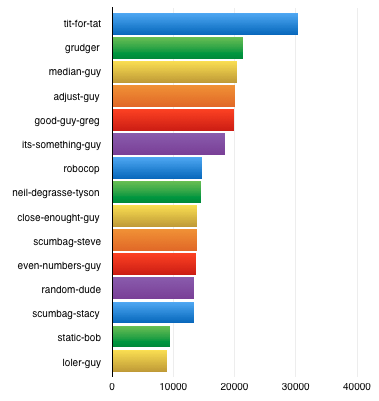
\includegraphics[scale=0.75, angle=0]{bilder/points.png}
	\caption{Detta är bildtexten}
	\label{points}
	\end{center}
\end{figure}

\begin{figure}[htb]
	\begin{center}
	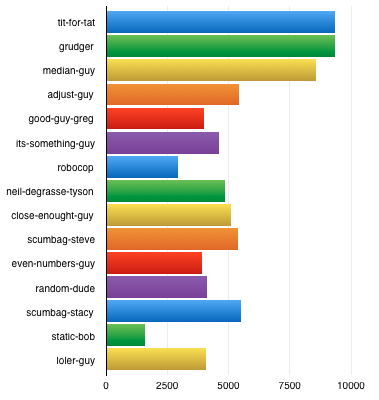
\includegraphics[scale=0.75, angle=0]{bilder/wins.png}
	\caption{Detta är bildtexten}
	\label{wins}
	\end{center}
\end{figure}



\newpage

\section{Diskussion}
\subsection{Resultat}

\subsection{Strategier}
Strategierna har utvecklats utav oss inom gruppen och har under projektets gång ifrågasatts en del. Vissa strategier har upplevts som meningslösa. I efterhand hade vi kunnat låta personer utanför projektgruppen skapa strategier, exempelvis som en tävling för att verkligen finna intressanta strategier, och framför allt fler strategier som tar hänsyn till resultathistoriken.

Grudger är en samarbetande strategi som belönar andra strategier som samarbetar, men straffar strategier som försöker maximera vinsten. Det gör att Grudger får bra poängutdelning mot strategier som också samarbetar(så som tit-for-tat, goog-guy-greg och sig själv). De strategier som försöker maximera sin egen vinst kommer Grudger att straffa genom att bara spela ettor. Det gör att Grudger kommer att erhålla poäng varje omgång så länge inte motståndaren också spelar ettor.  Om Grudger möter en strategi som också straffar sina motståndare så kommer båda dessa strategier att spela ettor. Detta resulterar i att ingen av strategierna kommer att få några poäng eftersom de spelar lika varje omgång. Exempel på detta beteende kan observeras när Grudger möter strategier som den inte lyckas få någon vinst mot så som loler-guy, median-guy med flera.

\begin{figure}[htb]
	\begin{center}
	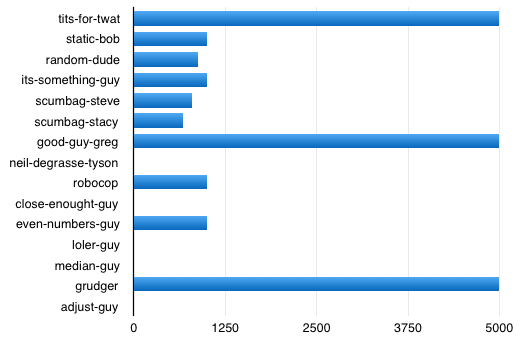
\includegraphics[scale=0.75, angle=0]{bilder/grudger.png}
	\caption{Detta är bildtexten}
	\label{grudger}
	\end{center}
\end{figure}

Den strategi som lyckats best i är tit for tat. I figur * syns det tydligt att tit for tat spelar bra mot majoriteten av de andra strategierna. De strategier som tit for tat har svårt mot är de som tvingar den andra strategin att tillslut bara spela ettor. Mot dessa kommer tit for tat bara att få några få poäng. Mot statiska strategier lyckas tit for tat hitta ett läge där den maximerar sin vinst. Detta gör att den har någorlunda stora vinster mot its something guy, robocop och static Bob.

\begin{figure}[htb]
	\begin{center}
	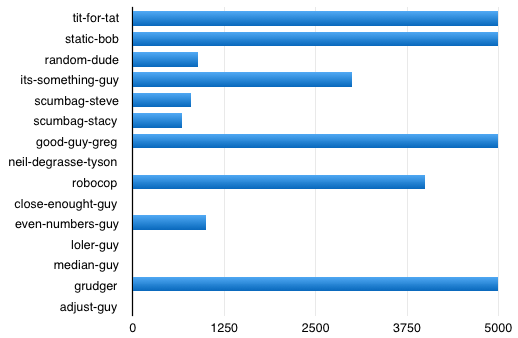
\includegraphics[scale=0.75, angle=0]{bilder/tit-for-tat.png}
	\caption{Detta är bildtexten}
	\label{tit-for-tat}
	\end{center}
\end{figure}

En strategi som får jämnast utdelning totalt sett är adjust guy. De enda strategier som adjust guy spelar dåligt mot är strategier som tvingar adjust guy att börja spela ettor, då låser sig båda strategierna på att spela just ettor. Men mot andra strategier kommer adjust guy att försöka maximera vinsten genom att då höja en nivå till nästa omgång.
\begin{figure}[htb]
	\begin{center}
	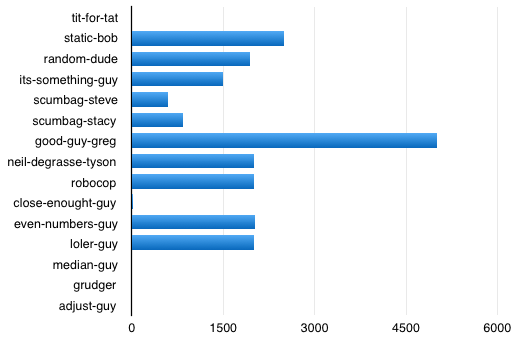
\includegraphics[scale=0.75, angle=0]{bilder/adjust-guy.png}
	\caption{Detta är bildtexten}
	\label{adjust-guy}
	\end{center}
\end{figure}
Anledningen till att good guy greg klarar sig så pass bra är att den vinner så mycket mot de strategier den faktiskt vinner mot. Det är strategier som nöjer sig med att spela tior, och inte försöker maximera sin vinst. Det gör att good guy greg inte skulle prestera särskilt bra om inte det fanns tillräckligt med sådana strategier.

\begin{figure}[htb]
	\begin{center}
	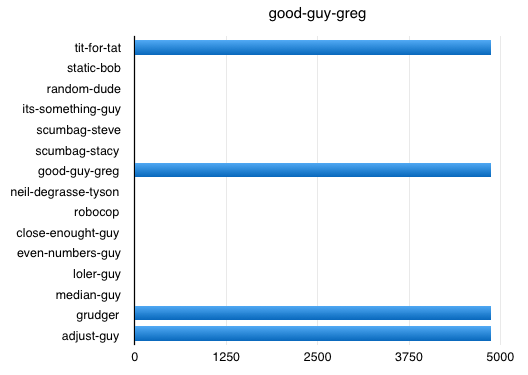
\includegraphics[scale=0.75, angle=0]{bilder/good-guy-greg.png}
	\caption{Detta är bildtexten}
	\label{good-guy-greg}
	\end{center}
\end{figure}

Median guy är en beräknande strategi. Dock spelar den bäst mot statiska strategier då den blir långsam att reagera mot strategier som alltid försöker lägga tidigare än sin motståndare. Dock kommer median guy att spela bra mot statiska strategier då den hittar vid vilket tidssteg motståndaren brukar välja och lägger sig under det. Den kommer även att spela förhållandevis bra mot strategier så som scumbag steve och scumbag stacy då median guy kommer hitta vilka värden de kör mest och sedan lägga sig under dessa.

\begin{figure}[htb]
	\begin{center}
	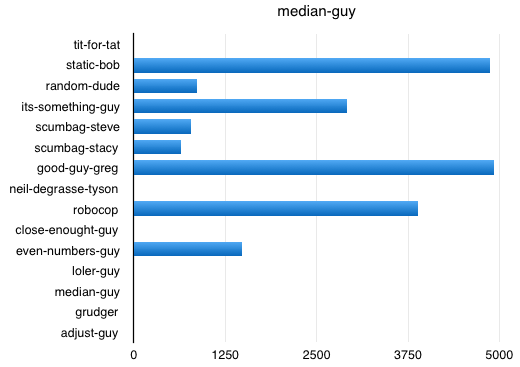
\includegraphics[scale=0.75, angle=0]{bilder/median-guy.png}
	\caption{Detta är bildtexten}
	\label{median-guy}
	\end{center}
\end{figure}


\noindent Ett intressant test som vi gjorde var att köra 10 strategier som släpper på varsitt tidssteg mot varandra flera gånger, dvs en strategi som släpper på 1, en som släpper på 2 och så vidare ända upp till 10. I detta test vann strategin som släppte på tidssteg 5 över tid. Strategi 4 och 6 hamnade på delad andra plats. Däremot så vann strategi nummer 1 över strategi nummer 5 i det “egentliga” testet. Därmet konstaterar vi att strategierna presterar väldigt olika beroende på vilka strategier som de möter.

\subsection{Projektet}
Gruppen har fungerat bra, och vi har följt tidsplanen och besvarat våra frågor. Vi kan emellertid tycka att vi skulle hittat relevant forskning i ett tidigare skede och utgå mer utifrån denna. Det var svårt att hitta artiklar som undersökt liknande frågeställningar. Vi tycker också att det var svårt att hitta vettiga problemformuleringar och frågeställningar inom just detta. Projektet startades egentligen bara med att vi diskuterade spelet och tyckte att det lät intressant att undersöka och då hamnade frågeställningarna i andrahand. Detta har inneburit att vi utvecklat vår medvetenhet gällande vad som krävs för att skriva vetenskapliga artiklar, där stor vikt skall läggas på tidigare forskning, samt formulerade av frågeställningar och hypoteser. I övrigt har projektet i sig har varit roligt att genomföra och har även gett oss ytterligare förståelse i framför allt game theory. 

\subsection{Framtida studier?}
Skall detta vara med också kanske??

%%%%% BEGIN OF 3rd ADJUSTMENTS SECTION %%%%%
% For the outline and annotated bibliography (deliverable 2)
% you must use the following two commands:
%
\nocite{*}  % Includes ALL entries from the .bib-file, even if they are
            % not '\cite{}'-ed in the text above
\bibliographystyle{plain-annote}
%
%For the full and final paper (deliverables 3 and 4a/b)
% use ONLY the following commands (i.e. put the commands above into
% comments and uncomment the command below):
%
% \bibliographystyle{splncs}
%
%%%%% END OF ADJUSTMENTS SECTION %%%%%

\bibliography{rapport}

\end{document}
